\section{Evaluation}

\subsection{Detailed evaluation of examples}

In this section we discuss in full detail the execution trace
of the implementation of some examples. 

\subsubsection{Symbol elimination example}

Let us consider the following example from \cite{KAPUR2017} 
$\alpha_1 = \{f(z_1, v) = s_1, f(z_2, v) = s_2, f(f(y_1, v), f(y_2, v)) = t\}$
with the set of symbols to eliminate $U_1 = \{v\}$. The implementation produces the following
trace (slightly modified for presentation purposes) in order to compute 
the interpolant of $\alpha_1; U_1$:

\verbatiminput{../../Software/Cpp/EUFInterpolant/tests/traces/current_progress_example1.txt}

%The interface offered by SMT solvers with interpolation features usually provide the 
%conventional A-part, B-part format. In order to compare the results with the implementation two 
%instances were tested, so we can obtain interpolants from both systems:

%\begin{itemize}
  %\item Problem instance: A-part : $\{f(z_1, v) = s_1, f(z_2, v) 
    %= s_2, f(f(y_1, v), f(y_2, v)) = t\}$; B-part : 
    %$\{z_1 = z_2, s_1 \neq s_2 \}$. Our implementation
    %computes the symbols to be eliminated to be $\{f, v, y_1, y_2\}$.
    %\begin{itemize}
      %\item Z3: (or (= s2 s1) (not (= z2 z1)))
      %\item Mathsat: (not (and (= z1 z2) (not (= s1 s2))))
      %\item Our implementation: ($\rightarrow$ (= z1 z2) (= s1 s2))
    %\end{itemize}

  %\item Problem instance: A-part : $\{f(z_1, v) = s_1, f(z_2, v) 
    %= s_2, f(f(y_1, v), f(y_2, v)) = t\}$; 
    %B-part : $\{z_1 = y_1, z_1 = y_2, f(s_1, s_1) \neq t\}$.
    %Our implementation
    %computes the symbols to be eliminated to be $\{s_2, z_2, v\}$.

    %\begin{itemize}
      %\item Z3: (or (= (f s1 s1) t) (not (= z1 y1)) (not (= y2 y1)))
      %\item Mathsat: (not (and (not (= t (f s1 s1))) (and (= z1 y1) (= z1 y2))))
      %\item Our implementation: ($\rightarrow$ (and (= y1 y2) (= z1 y2) (= z1 y2)) (= t (f s1 s1))))
  %\end{itemize}

%\end{itemize}

%Clearly, the interpolant obtained by just eliminating the symbol $v$ implies
%the outputs produced by Z3 and Mathsat for the previous problem instances.

The final output of our implementation is 
$(((z_1 = y_1) \land (z_1 = y_2) \land (z_1 = y_1) \land (z_2 = y_1)) \rightarrow (t = f(s_1, s_2))) \land
((z_1 = z_2) \rightarrow (s_1 = s_2)) \land
(((z_2 = y_1) \land (z_1 = y_2) \land (z_1 = y_1) \land (z_2 = y_1)) \rightarrow (t = f(s_2, s_2))) \land
(((z_2 = y_1) \land (z_1 = y_2)) \rightarrow (t = f(s_2, s_1))) \land
(((z_1 = y_1) \land (z_1 = y_2)) \rightarrow (t = f(s_1, s_1)))$.

\subsubsection{Simple example with dis-equality}

Let us consider another example from \cite{KAPUR2017} 
$\alpha_2 = \{f(x_1) \neq f(x_2)\}$
with the set of symbols to eliminate $U_2 = \{f\}$. The implementation produces the following
trace for $\alpha_2; U_2$:

\verbatiminput{../../Software/Cpp/EUFInterpolant/tests/traces/current_progress_example2.txt}

The final output of our implementation is $x_1 = x_2 \rightarrow \bot$.

%To compare our result with Z3 and Mathsat we 
%included the B-part formula to be $\{x_1 = x_2\}$.
%The interpolants obtained by these systems were the 
%same, which was (not (= x1 x2)).

\subsubsection{Comparison of Interpolants and Uniform Interpolants}

In this section we compare the Craig Interpolants obtained by Z3 and Mathsat for contradicting pairs of formulas and the uniform interpolant obtained by our implementation such
that the symbols to eliminate are the same
for each input problem for our implementation.

\begin{table}[h]
\centering
\begin{tabular}{ccc}
\toprule
\multicolumn{3}{c}{A-part: $f(z_1, v) = s_1 \land f(z_2, v) = s_2 \land f(f(y_1, v), f(y_2, v)) = t$} \\
\midrule 
{} & \multicolumn{2}{c}{B-parts} \\
\cmidrule{2-3} \\
{} & 
\makecell{$z_1 = z_2 \land z_2 = y_1$ \\ $\land z_2 = y_2 \land f(s_2, s_1) \neq t$} & 
\makecell{$z_1 = z_2 \land z_1 = y_1$ \\ $\land z_2 = y_2 \land f(s_1, s_2) \neq t$} \\
\midrule
\multirow{1}{*}{SMT Solvers} & \multicolumn{2}{c}{Interpolants} \\
\midrule
Z3 & 
\makecell{$((f(s_2, s_1) = t) \lor (\neg (z_2 = z_1))$ \\ $\lor ((\neg (s_1 = s_2)) \land ((s_2 = s_1) \lor$ \\ $(\neg (z_2 = z_1)))) \lor (\neg (y_1 = z_1))$ \\ $\lor (\neg (y_2 = z_1)))$} & 
\makecell{$((f(s_1, s_2) = t) \lor ((\neg (s_1 = s_2))$ \\ $\land ((s_2 = s_1) \lor (\neg (z_2 = z_1)))) \lor$ \\ $(\neg (z_2 = z_1)) \lor (\neg (y_1 = z_1))$ \\ $\lor (\neg (y_2 = z_1)))$} \\
\midrule
Mathsat & 
\makecell{$\neg ((\neg (t = f(s_2, s_1))) \land ((= z_2 y_1)$ \\ $\land ((= z_1 z_2) \land (= z_2 y_2))))$} & 
\makecell{$\neg ((\neg (t = f(s_1, s_2))) \land (((= z_1 z_2)$ \\ $ \land (= z_1 y_1)) \land (= z_1 y_2)))$}\\
\bottomrule
\end{tabular}
\end{table}

TODO: keep working here. Just mention that the output produced by our implementation is X and that X was stronger.

%%% Local Variables:
%%% mode: latex
%%% TeX-master: "main"
%%% End:


\subsection{Performance comparison with iZ3 and MathSat}\label{performance_euf}

This section discusses a benchmark of interpolant generation
for the EUF theory, which it will allow us to test 
our implementation and contrast the execution 
time with other interpolant generation
algorithms from Z3 and Mathsat.

\subsubsection{Benchmark description}

The benchmark uses the following parameters:

\begin{itemize}
  \item $i$ stands for the number of constants
  \item $j$ stands for the number of function symbols
    with arity between 2 and 3
  \item $k$ stands for limit for random terms to consider
    in the problem
  \item $n$ stands for the equations/dis-equations in the
    A-part
\end{itemize}

The benchmark generates a pair of two unsatisfiable formulas
in the EUF language from a fixed theory with the following parameters:

\begin{equation*}
  S = \{ c_1, \dots, c_i, f_1, \dots, f_j \}
\end{equation*}

where $i, j$ are random integer numbers. Using the $S$, we
enumerate the grounded terms $G$ in $S$ and assign a natural 
number to each number denoting its position in the enumeration.

We generate $n$ random equations/dis-equations from the signature $S$ 
such that this
collection of formulas is consistent for the $A-part$ of
the input problem. 
The latter is implemented using a $z3: :solver$ to ensure 
this condition.
The equations/dis-equations are of the form:

\begin{equation*}
  position(k_1, S) = position(k_2, S) \text{ , or } position(k_1, S) \neq position(k_2, S) 
\end{equation*}

where $position(k, S)$ denotes the $k^{th}$ element in $G$. The 
integers $k_1, k_2$ are chosen uniformly at random from a
distribution of integer values $\{0, \dots, k\}$, 
where $k$ is a parameter of the benchmark.

Next we randomly generate a second set of consistent 
equations/dis-equations (B-Part) until the $A-part$ and the
$B-part$ are inconsistent using a second $z3: :solver$.

\begin{figure}[!ht]
  \centering
  \begin{BVerbatim}[fontsize=\tiny]
    A part formulas:
    (ast-vector
      (distinct (f_0 x_6 x_0 x_0 x_0) (f_0 x_9 x_8 x_0 x_0))
      (= (f_0 x_8 x_1 x_0 x_0) (f_0 x_1 x_0 x_0 x_0))
      (= (f_0 x_5 x_2 x_0 x_0) (f_0 x_4 x_5 x_0 x_0))
      (distinct (f_0 x_6 x_2 x_0 x_0) (f_0 x_9 x_3 x_0 x_0))
      (distinct (f_0 x_4 x_7 x_0 x_0) x_7)
      (= (f_0 x_5 x_5 x_0 x_0) (f_0 x_8 x_1 x_0 x_0))
      (= (f_0 x_2 x_6 x_0 x_0) (f_0 x_9 x_3 x_0 x_0))
      (= x_7 (f_0 x_1 x_6 x_0 x_0))
      (= (f_0 x_1 x_4 x_0 x_0) (f_0 x_6 x_3 x_0 x_0))
    (= x_8 (f_0 x_2 x_6 x_0 x_0)))
    B part formulas:
    (ast-vector
      (= (f_0 x_6 x_8 x_0 x_0) (f_0 x_9 x_7 x_0 x_0))
      (distinct (f_0 x_2 x_6 x_0 x_0) (f_0 x_7 x_0 x_0 x_0))
      (distinct (f_0 x_7 x_7 x_0 x_0) x_4)
      (distinct (f_0 x_6 x_6 x_0 x_0) (f_0 x_3 x_8 x_0 x_0))
      (= (f_0 x_2 x_5 x_0 x_0) (f_0 x_7 x_6 x_0 x_0))
      (= (f_0 x_6 x_0 x_0 x_0) (f_0 x_2 x_3 x_0 x_0))
      (= (f_0 x_3 x_3 x_0 x_0) (f_0 x_6 x_5 x_0 x_0))
      (distinct (f_0 x_8 x_8 x_0 x_0) (f_0 x_5 x_1 x_0 x_0))
      (distinct (f_0 x_7 x_8 x_0 x_0) (f_0 x_9 x_1 x_0 x_0))
      (= (f_0 x_8 x_8 x_0 x_0) (f_0 x_7 x_2 x_0 x_0))
      (distinct (f_0 x_2 x_1 x_0 x_0) (f_0 x_3 x_2 x_0 x_0))
      (= (f_0 x_5 x_3 x_0 x_0) (f_0 x_7 x_4 x_0 x_0))
      (distinct (f_0 x_1 x_2 x_0 x_0) (f_0 x_5 x_3 x_0 x_0))
      (= (f_0 x_1 x_7 x_0 x_0) (f_0 x_3 x_6 x_0 x_0))
      (distinct (f_0 x_3 x_2 x_0 x_0) (f_0 x_8 x_7 x_0 x_0))
      (= (f_0 x_2 x_8 x_0 x_0) x_4)
      (= (f_0 x_2 x_2 x_0 x_0) (f_0 x_8 x_3 x_0 x_0))
      (= (f_0 x_1 x_1 x_0 x_0) (f_0 x_8 x_8 x_0 x_0))
      (distinct (f_0 x_3 x_2 x_0 x_0) (f_0 x_8 x_3 x_0 x_0))
      (= (f_0 x_2 x_8 x_0 x_0) (f_0 x_6 x_3 x_0 x_0))
      (distinct (f_0 x_5 x_6 x_0 x_0) (f_0 x_0 x_1 x_0 x_0))
      (= (f_0 x_7 x_3 x_0 x_0) (f_0 x_7 x_0 x_0 x_0))
      (distinct (f_0 x_0 x_3 x_0 x_0) (f_0 x_8 x_3 x_0 x_0))
      (distinct (f_0 x_8 x_2 x_0 x_0) (f_0 x_2 x_7 x_0 x_0))
      (distinct (f_0 x_9 x_1 x_0 x_0) (f_0 x_5 x_0 x_0 x_0))
      (distinct (f_0 x_0 x_4 x_0 x_0) (f_0 x_0 x_5 x_0 x_0))
      (distinct (f_0 x_5 x_5 x_0 x_0) (f_0 x_2 x_8 x_0 x_0))
      (= (f_0 x_6 x_3 x_0 x_0) (f_0 x_3 x_0 x_0 x_0))
      (= (f_0 x_3 x_8 x_0 x_0) (f_0 x_0 x_8 x_0 x_0))
      (distinct (f_0 x_8 x_0 x_0 x_0) (f_0 x_5 x_5 x_0 x_0))
      (= (f_0 x_6 x_6 x_0 x_0) (f_0 x_4 x_5 x_0 x_0))
      (distinct (f_0 x_4 x_3 x_0 x_0) x_5)
      (distinct x_8 (f_0 x_3 x_3 x_0 x_0))
      (= (f_0 x_6 x_3 x_0 x_0) (f_0 x_3 x_6 x_0 x_0))
      (= (f_0 x_4 x_1 x_0 x_0) (f_0 x_5 x_6 x_0 x_0))
      (= x_7 (f_0 x_0 x_3 x_0 x_0))
      (distinct (f_0 x_1 x_3 x_0 x_0) (f_0 x_8 x_2 x_0 x_0))
      (= (f_0 x_2 x_1 x_0 x_0) (f_0 x_6 x_8 x_0 x_0))
      (= x_3 (f_0 x_9 x_7 x_0 x_0))
      (= (f_0 x_3 x_7 x_0 x_0) x_8)
    (= (f_0 x_3 x_7 x_0 x_0) (f_0 x_6 x_2 x_0 x_0)))
  \end{BVerbatim}
  \caption{Typical example of benchmark used}
\end{figure}

\subsubsection{Experimental results}

We designed this problem because it is not trivial to 
compute a  uniform/interpolant due to randomness of the
problem. This problem was executed $100$ times
with parameters (i = 10, j = 5, k = 100, n = 10) and 
(i = 20, j = 10, k = 100, n = 40)
using a computer desktop
equipped with an Intel i7-9700 @ 4.70 GHz processor 
and 16 GB of RAM. 

The following graph reports the time needed
by our implementation, iZ3, and the interpolation 
generation algorithm from Mathsat. 
It is well known that both iZ3 and Mathsat does not
compute uniform interpolants. Regardless, the benchmark
was used with the purpose to compare their execution time
on normal interpolants.

The time was
measured using a bash script which takes the difference
of the output produced by the UNIX utility $date +`\%s.\%N'$ 
at the beginning and at the end of the execution of the 
tested algorithms.

\begin{figure}
  \centering
  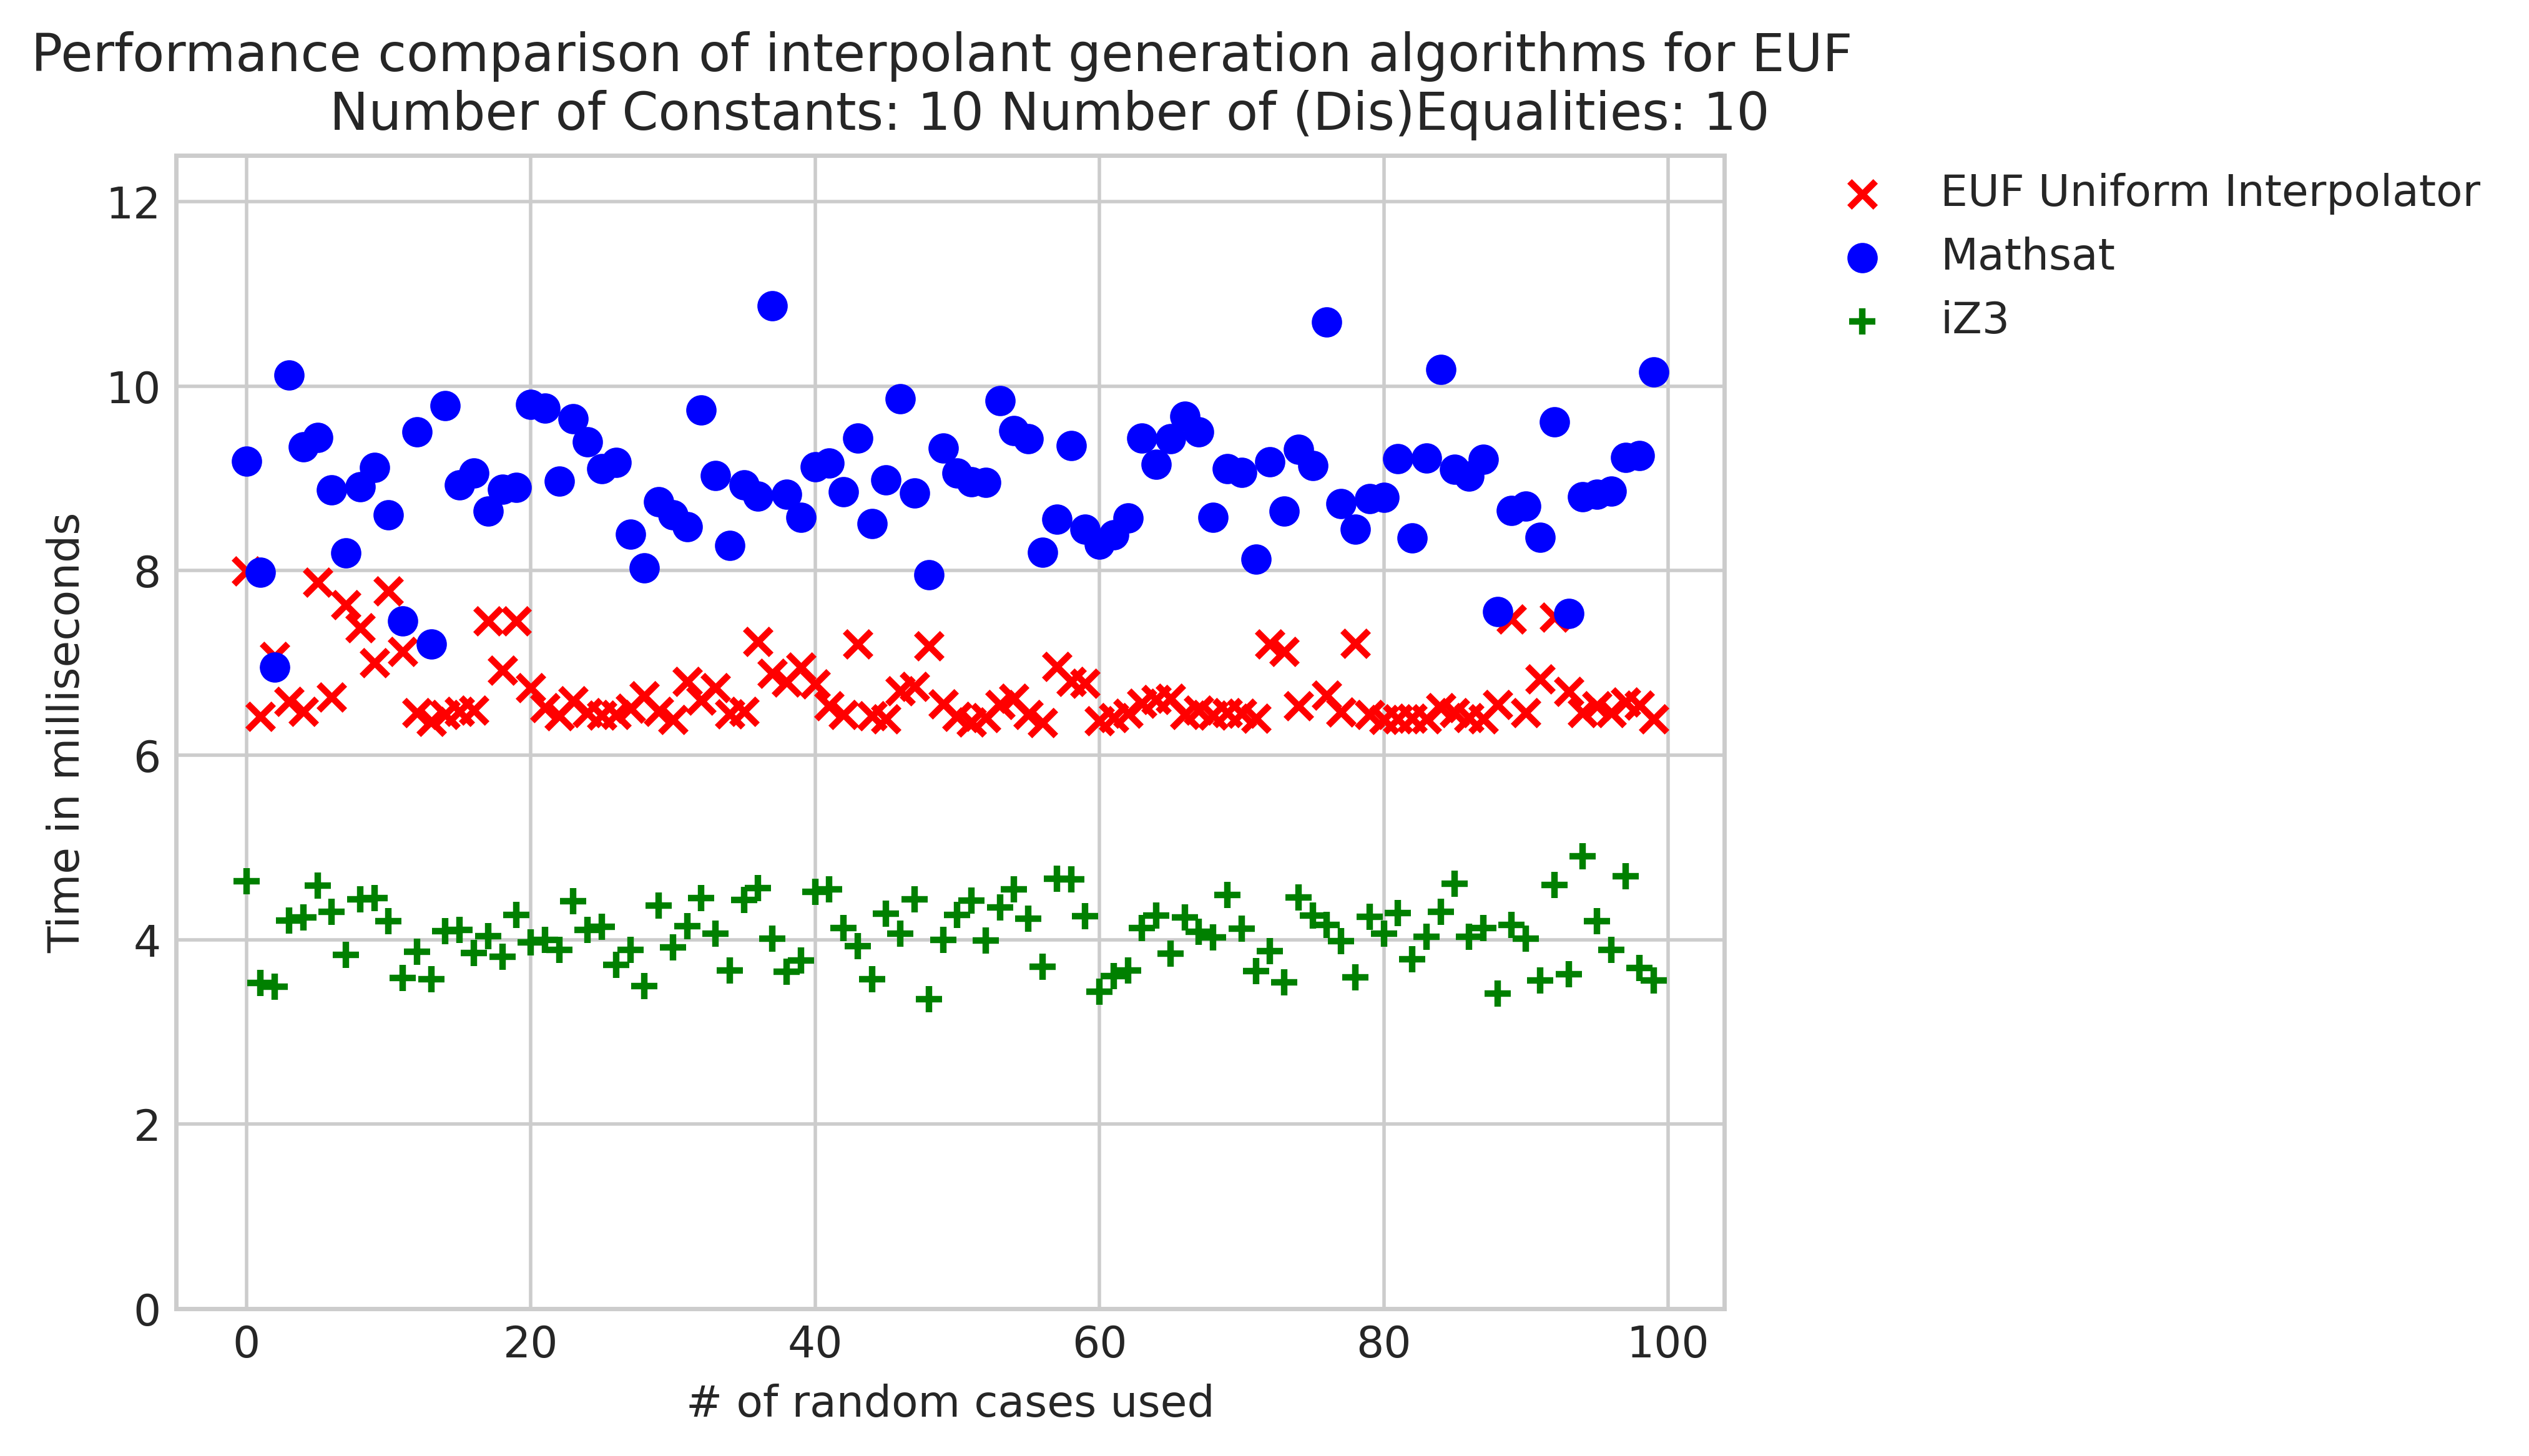
\includegraphics[scale=0.9]{figures/eufi_performance_graph_10_5_3_10_100}
  \caption{Performance comparison graph of EUF interpolant generation
  algorithms for the benchmark (i = 10, j = 5, k = 100, n = 10)}
  \label{performance_graph_euf}
\end{figure}

\begin{figure}
  \centering
  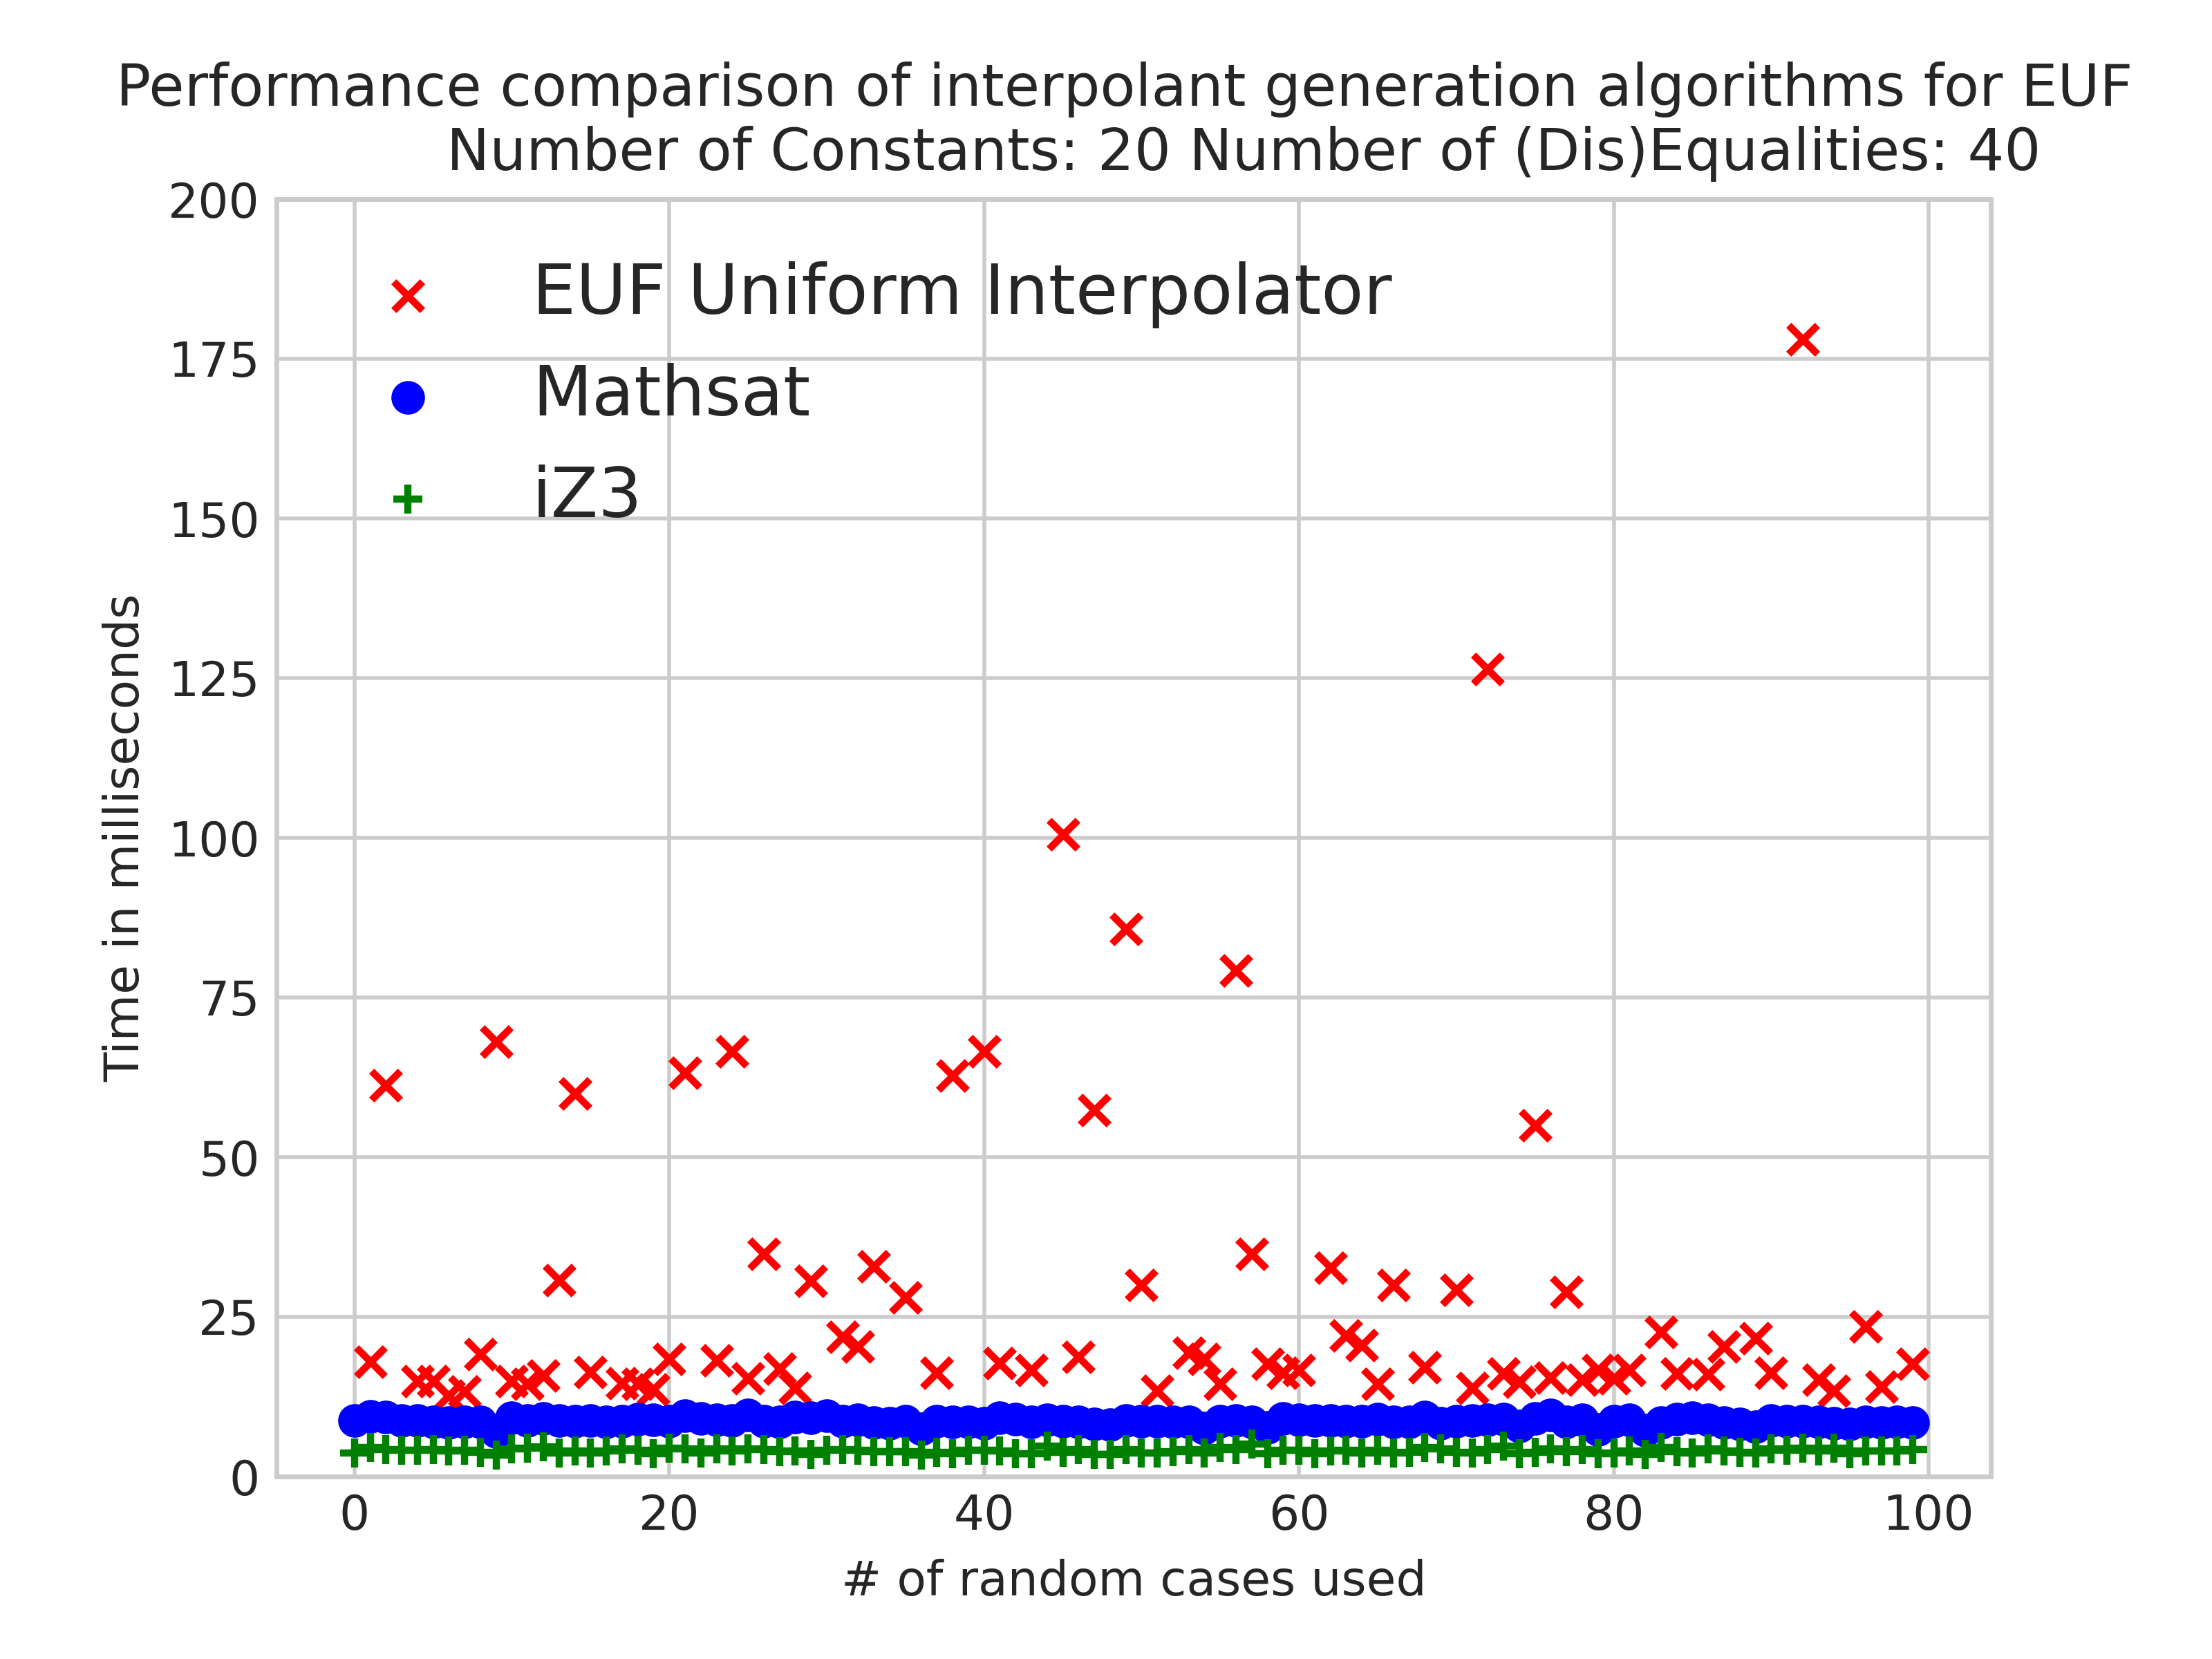
\includegraphics[scale=0.9]{figures/eufi_performance_graph_20_10_3_40_100}
  \caption{Performance comparison graph of EUF interpolant generation
  algorithms for the benchmark (i = 20, j = 10, k = 100, n = 40)} 

  \label{performance_graph_euf_2}
\end{figure}

%%% Local Variables:
%%% mode: latex
%%% TeX-master: "main"
%%% End:


%%% Local Variables:
%%% mode: latex
%%% TeX-master: "main"
%%% End:
